
\documentclass[12pt,a4paper]{article}

%======Usepackage=========
\usepackage[utf8]{inputenc}
\usepackage[ngerman]{babel}
\usepackage{graphicx}
\usepackage{hyperref}
\usepackage[square,sort,comma,numbers]{natbib}
\usepackage{tabularx}
\usepackage{fancyhdr}
\usepackage[T1]{fontenc}
\usepackage{lscape}
\usepackage[onehalfspacing]{setspace}
\usepackage{amssymb}
\usepackage{amsmath}
\usepackage[locale=DE]{siunitx}
\usepackage[printonlyused]{acronym}
\usepackage[table]{xcolor}
\usepackage{eurosym}
\usepackage{listings}
\usepackage{pdfpages}

\lstdefinestyle{customc}{
numbers  = left,
numberstyle=\tiny,
numbersep=5pt,
numberblanklines=true,
basicstyle=\sffamily\small,
frame=lines,
showstringspaces = false,
  %belowcaptionskip=1\baselineskip,
  breaklines=true,
  %frame=L,
  xleftmargin=\parindent,
  %language=java,
  %showstringspaces=false,
  %basicstyle=\footnotesize\ttfamily,
  keywordstyle=\bfseries\color{green!40!black},
  commentstyle=\itshape\color{purple!40!black},
  identifierstyle=\color{blue},
  stringstyle=\color{orange},
  abovecaptionskip=\baselineskip,
  captionpos=b
}

%=====Allgemeine Angaben======
\title{Bachelorarbeit}
\author{Marvin Böck}
\date{\today}
\newcommand{\Autor}{Marvin Böck}
\newcommand{\MatrikelNummer}{1892597}
\newcommand{\Kursbezeichnung}{Tinf18B3}


\newcommand{\FirmenName}{SICK STEGMANN GmbH}
\newcommand{\FirmenLogoDeckblatt}{
\includegraphics[width=3cm]{img/Sick_logo.png}}
\newcommand{\FirmenStadt}{Donaueschingen}
\newcommand{\BetreuerFirma}{Timo Bayer, M.Sc.}
\newcommand{\BetreuerDHBW}{Prof. Dr. Hans-Jörg Haubner}
\newcommand{\Titel}{Konzeption und Implementierung einer modularen Testsuite
zur Automatisierung von Softwaretests}
\newcommand{\Untertitel}{Test}
\newcommand{\ModulName}{B-FMP02XX}
\newcommand{\AbgabeDatum}{07. Juli 2022}

\newcommand{\Dauer}{6. Praxisphase}
\newcommand{\Abschluss}{Bachelor of Science}

\newcommand{\Studiengang}{Informatik / Informationstechnik}
\newcommand{\Anschrift}{Solweg 5, 78647 Trossingen}

%======Kopf/Fußzeile=====
\pagestyle{fancy}

    \lhead{}
    \chead{}
    \rhead{\slshape \leftmark}

    \lfoot{}
    \cfoot{\thepage}
    \rfoot{}
    
    \renewcommand{\headrulewidth}{0.4pt}
    \renewcommand{\footrulewidth}{0.4pt}


\bibliographystyle{IEEEtran}    
%======Dokument=======
\begin{document}

%=====deckblatt, Abstrackz/Verzeichnisse======
\pagestyle{empty}
%%\maketitle
\singlespacing
\begin{center}
%\hspace{-2mm} 
\includegraphics[scale=0.15]{img/wbh_logo.jpg}
\FirmenLogoDeckblatt\hfill
\includegraphics[width=4cm]{img/wbh_logo.jpg}\\[2cm]
{\Huge \Titel}\\[1cm]
%{\Huge\scshape \Was}\\[1cm]
{\large für die Prüfung zum}\\[0.5cm]
{\Large \Abschluss}\\[0.5cm]
{\large des Studienganges \Studiengang}\\[0.5cm]
{\large an der}\\[0.5cm]
{\large Dualen Hochschule Baden-Württemberg Karlsruhe}\\[0.5cm]
{\large von}\\[0.5cm]
{\large\bfseries \Autor}\\[1cm]
{\large Abgabedatum \AbgabeDatum}
\vfill

\begin{tabular}{l@{\hspace{2cm}}l}
Bearbeitungszeitraum	         & \Dauer 			\\
Matrikelnummer	                 & \MatrikelNummer		\\
Kurs			         & \Kursbezeichnung		\\
Ausbildungsfirma	         & \FirmenName			\\
			         & \FirmenStadt			\\
Betreuer der Ausbildungsfirma	 & \BetreuerFirma		\\
Gutachter der Studienakademie	 & \BetreuerDHBW		\\
\end{tabular}
\end{center}
 %Für große Arbeiten wie z.B. Masterthesis
%\maketitle
\singlespacing
\begin{center}
%\FirmenLogoDeckblatt\hfill
\includegraphics[width=4cm]{img/wbh_logo.jpg}\\[2cm]
\hfill
\includegraphics[width=4cm]{img/wbh_logo.jpg}\\[2cm]
{\Huge \Titel}\\[1cm]
%{\Huge\scshape \Was}\\[1cm]
{\Large \Untertitel}\\[0.5cm]
{\Large Fachbereich Informatik}\\[0.5cm]
{\large \ModulName}\\[0.5cm]

\vfill

\begin{tabular}{l@{\hspace{2cm}}l}
Autor	 & \Autor		\\
Matrikelnummer	                 & \MatrikelNummer		\\
Anschrift 	& \Anschrift \\
Abgabedatum	 & \AbgabeDatum		\\

\end{tabular}
\end{center}
 %Für kleine Arbeiten, Berichte etc.
\pagenumbering{Roman}
\onehalfspacing
\section*{Erklärung an Eidesstatt}

Hiermit erkläre ich, dass ich die vorliegende Abschlussarbeit mit dem Titel:
\newline
	''\textit{\Titel{}}''
\newline
eigenständig und ohne fremde Hilfe angefertigt habe. Textpassagen, die wörtlich oder dem Sinn nach auf Publikationen oder Vorträgen anderer Autoren beruhen, sind als solche kenntlich gemacht. Die Arbeit wurde bisher keiner anderen Prüfungsbehörde vorgelegt und auch noch nicht veröffentlicht.
\newline
Ich versichere zudem, dass die eingereichte elektronische Fassung mit der gedruckten
Fassung übereinstimmt.

\vspace{4cm}
\parbox{5cm}{\centering \dotfill\\
\centering \footnotesize Ort, Datum} \hfill\parbox{5cm}{\dotfill\\
\centering \footnotesize Unterschrift}



\section*{Sperrvermerk}
Der Inhalt der Arbeit darf weder als Ganzes noch in Auszügen Personen außerhalb des Prüfungsprozesses und des Evaluationsverfahrens zugänglich gemacht werden, sofern keine anderslautende Genehmigung der SICK STEGMANN GmbH vorliegt
\newline


\onehalfspacing
\section*{Zusammenfassung}
Die vorliegende Arbeit befasst sich mit der Kozeptionierung sowie Proof of Concept Implementierung einer modularen Testsuite für Softwaretests. Grund für die Entwicklung der Suite ist die Portierung eines Bestandsprodukts auf eine neue Mikrocontroller Generation und der damit verbundener erhöhter Testaufwand. Bei der Firma SICK STEGAMNN GmbH ist seit kurzem ein Framework zum automatischen Testen von Software im Einsatz welches die Möglichkeit bietet, entsprechende Softwaretests komfortabel abzudecken. Um die Generierung der Testfälle für das Portierungsprojekt zu erleichtern, soll im Rahmen dieser Arbeit eine Testsuite konzeptioniert, sowie prototypisch implementiert werden. Ziel hierbei ist es, den späteren Prozess der Testentwicklung zu beschleunigen, sowie die Testfiles übersichtlicher und robuster zu gestalten. Zu Beginn der Arbeit wird sich ein Überblick über den Bereich Automated Testing @ GBC07 sowie Software Tests im Embedded Bereich geschaffen. Im Anschluss daran, werden die Testfälle eines vergleichbaren Produkts analysiert und geeignete Testfälle identifiziert. Danach wird eine Softwarearchitektur für die Suite konzeptioniert und diese prototypisch implementiert. Zum Schluss werden die Ergebnisse der Arbeit evaluiert.
\newpage
\section*{Abstract}
This thesis deals with the conceptual design and proof of concept implementation of a modular test suite for software testing. The reason for the development of the suite is the porting of an existing product to a new microcontroller generation and the associated increased test effort. The company SICK STEGAMNN GmbH has recently implemented a framework for automatic software testing which offers the possibility to comfortably cover the corresponding software tests. In order to facilitate the generation of test cases for the porting project, a test suite is to be conceptualized and prototypically implemented within the scope of this work. The goal is to accelerate the later process of test development and to make the test files clearer and more robust. At the beginning of the work, an overview of the area of Automated Testing @ GBC07 and software tests in the embedded area is created. Subsequently, the test cases of a comparable product are analyzed and suitable test cases are identified. Afterwards a software architecture for the suite is conceptualized and prototypically implemented. Finally, the results of the work are evaluated.


\singlespacing
%=====Inhaltsverzeichniss===
\tableofcontents
\newpage
%====Abbildungsverzeichniss===
\listoffigures
\newpage
%====Tabellenverzeichniss===
\listoftables
\newpage
%====Listings====
\lstlistoflistings
\newpage
%===Abkürzungsverzeichnis===
\newpage
\section*{Abkürzungsverzeichnis}
	\begin{acronym}[slmtA]
		\acro{MFB}{Motor-Feedback-System}
		\acro{SRS}{Software Requirements Specification}
		\acro{RUP}{Rational Unified Process}
		\acro{CCE}{Continuous and Customised Engineering}
		\acro{LOC}{Lines of Code}
	\end{acronym}

%====Text=============
\newpage
\pagenumbering{arabic}
\pagestyle{fancy}
\newpage
\onehalfspacing

\section{Einleitung}

		\subsection{SICK}

\onehalfspacing
\section{Related Work}
In diesem Kapitel werden verschiedene Literaturquellen diskutiert, welche im Zusammenhang mit dem Thema der Arbeit stehen. Hierbei wird der Inhalt kurz zusammengefasst und erläutert, in welchem Zusammenhang die Arbeiten stehen.
\subsection*{Optimized test suites for automated testing using different optimization techniques}
In diesem Artikel, welcher von Manju Khari, Prabhat Kumar, Daniel Burgos und Rubén González Crespo geschrieben wurde, befassen sich die Autoren mit der Optimierung von automatisierten Testsuites unter Betrachtung verschiedener Optimierungstechniken. Hierbei werden Tools zur automatischen Generierung von Testsuites verglichen. Die Ergebnisse werden dann im Kontext des Automated Testing betrachtet. Die Arbeit zeigt auf, welche Möglichkeiten bei der Optimierung und automatischen Generierung von Softwaretests bestehen. Im Zuge des konkreten Projekts wird ebenfalls eine Testsuite erstellt. Die Betrachtung von eventuellen Optimierungsmöglichkeiten ist für den späteren Verlauf des Projekts durchaus von Interesse.\cite{ManjuKhariPrabhatKumarDanielBurgosRubenGonzalezCrespo.2017}

\subsection*{Eine Technologe für das durchgängige und automatisierte testen eingebetteter Software}
Die Arbeit, welche durch Dipl.-Inform. Till Fischer im Rahmen seiner Dissertation an der Fakultät für Elektrotechnik und Informationstechnik des Karlsruher Instituts für Technologie (KIT)durchgeführt wurde, werden neben den Grundlagen des Testens von eingebetteten Systemen auch die verschiedenen Testebenen diskutiert. Ziel der Arbeit ist die Verbesserung der Durchgängigkeit des Testprozesses für eingebettete Systeme. Als Lösungsstrategie wird durch Fischer eine Testlösung versiert, welche den Quelltext der ausgeführten Software, die Netzwerkkommunikation, sowie das physikalische Verhalten an elektrischen Schnittstellen und der simulierten Umgebung abdeckt. Hier ist der Bezug zum in dieser Arbeit behandelten Automated Testing @ GBC07 Projekt zu erkennen. \cite{Dipl.Inform.TillFischer.2016}



\onehalfspacing
\section{Grundlagen Softwareentwicklung und Verifikation}

%\onehalfspacing
\section{Anforderungen}
	\subsection{Anforderungsdefinition}
Zu Beginn des Projekts werden die konkreten Anforderungen an die Suite mit dem Auftraggeber abgestimmt und in Form einer Tabelle Festgehalten. Dieses Vorgehen erleichtert die Endabnahme des Projekts, da die Anforderungen klar definiert und beiden Parteien bekannt sind. Auf die Erstellung eines gesamten \ac{SRS} wird im Rahmen dieses Projekt aus Zeitgründen bewusst verzichtet. Bei den Anforderungen wird zwischen funktionalen und nicht-funktionalen unterschieden. Funktionale Anforderungen sind all jene, welche eine konkrete Funktion der Software definieren. Nicht Funktionale Anforderungen sind Anforderungen wie z.B. Zuverlässigkeit und Zeitverhalten. Die Anforderungen sind in den Tabellen \dq \nameref{tab:Anforderungstabelle}\dq und \dq \nameref{tab:Anforderungstabelle2}\dq dargestellt.
\newpage
\begin{table}[h]
\begin{center}
\begin{tabularx}{\textwidth}{|c|X|X|c|}
\hline
Nr. & Bezeichnung & Beschreibung & Zuordnung \\
\hline
F01 & Error Codes & Eignung zur Stimulation der verschiedenen Fehlerfälle und  dadurch Produktion der entsprechenden Fehlermeldungen (01h-23h) & Funktional \\
\hline
F02 & Identifikation des DUT & Überprüfung der Firmware Version, des elektronischen Typenschilds auf Korrektheit & Funktional \\
\hline
F03 & Diagnose Funktionalität & Überprüfung der vorhandenen Diagnose Funktionalität (z.B. Spannungs Monitoring) & Funktional \\
\hline
F04 & Core Funktionalität & Prüfung der externen Temperatur Schnittstelle, sowie der Single und multiturn Positionsbestimmung & Funktional \\
\hline
F05 & Schnittstellen Config & Auslesen und überprüfen der Schnittstellen Parametrisierung und Funktionalität & Funktional \\
\hline
F06 & Hiperface Befehle & Überprüfung der Funktion der verschiedenen Hiperface Befehle sowie der entsprechnden Antwort & Funktional \\
\hline
F07 & Integration in Automated Testing & Die Suite muss in das Projekt "Automated Testing" Integrierbar sein (Implementierung in ITE, Aufbau nach Vorgaben des Projekts) & Funktional \\
\hline
\end{tabularx}
\end{center}
\caption{Anforderungen funktional \label{tab:Anforderungstabelle}}
\end{table}

\begin{table}[h]

\begin{center}

\begin{tabularx}{\textwidth}{|c|X|X|c|}

\hline
Nr. & Bezeichnung & Beschreibung & Zuordnung \\
\hline
NF01 & Externes Equipment & Möglichkeit zur Integration des am Teststand vorhandenen externe Equipment & Nicht Funktional \\
\hline
NF02 & Universell einsetzbar & Der Aufbau der Suite soll so gestaltet sein, das diese auch zukünftig für die Portierung anderer (ähnlicher) Produkte genutzt werden kann & Nicht Funktional \\
\hline
NF03 & Coding Guidelines & Der Aufbau der Suite soll so gestaltet sein, das diese auch zukünftig für die Portierung anderer (ähnlicher) Produkte genutzt werden kann & Nicht Funktional \\
\hline


\end{tabularx}
\caption{Anforderungen nicht-funktional \label{tab:Anforderungstabelle2}}
\end{center}
\end{table}
\cleardoublepage

\subsection{Analyse bisheriger Testfälle}
Zu Ermittlung der Testfälle welche durch die Suite abgedeckt werden sollen werden die bisherigen Testpläne analysiert. Schwierigkeit hierbei ist, dass der Geber vor ca. 20 Jahren entwickelt wurde. Zum Entwicklungszeitpunkt fand keine, den heutigen Standards entsprechende Dokumentation der Testfälle (Testplan) statt, weiterhin ist zum Projektstart noch kein Testplan für Portierung des Controllers vorhanden. Aus diesem Grund wird für die Analyse der Testfälle auf den Testplan eines ähnlichen Produktes (SEY) welches ebenfalls über eine Hiperface Schnittstelle verfügt zurück gegriffen.\newline
	Die im Testplan festgelegten Tests werden in eine Excel Tabelle übertragen, die Testfälle sind im Testplan in verschiedene Kategorien unterteilt (z.B. General Requirements, HW Architecture, functional Requirements). Da der SEY über zwei Mikrocontroller verfügt (Master und Slave) der SK jedoch nicht werden daraufhin die Testfälle des Slave Microcontrollers aus dem Testplan gestrichen. In einem Zweite Schritt wird die Beschreibung jedes Testfalls Analysiert und geprüft ob dieser Testfall automatisierbar ist. Ein Beispiel für einen nicht automatisierbaren Testfall ist z.B. beim Eingriff mittels Debugger während des Tests gegeben. Die verbleibenden Tests werden mit dem Zuständigen SW-Entwickler besprochen und ggf. angepasst um im folgenden als Grundlage für die Kozeptionierung dienen zu können. Die Entwicklung eines kompletten Testplans für die Portierung wird hierbei nicht forciert, da hierzu der Zeitliche Rahmen nicht gegeben ist. Die 
Analyse der Testfälle zeigt, das sich die Suite besonders für das Testen der Hiperface Schnittstelle eignet. Hier können die verschiedenen Befehle der Schnittstelle gut abgebildet werden. Die Ergebnisse der Analyse sind in \dq \nameref{fig:Analyse.jpg}\dq   Beispielhaft dargestellt und befinden sich im Anhang. Die Farbgebung der Tabelle entspricht den Testfall Clustern.
\begin{figure}[h]
	\centering
  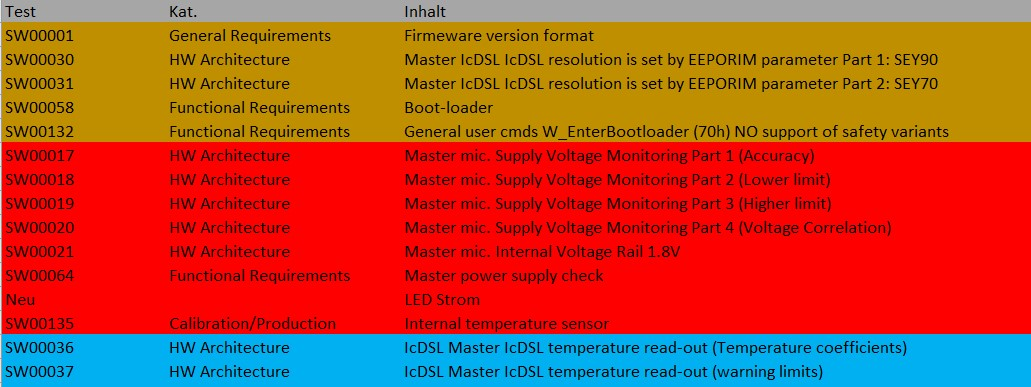
\includegraphics[width=1.25\textwidth, angle=90]{img/Tests_Cluster.jpg} 
   \caption{Tabelle mit Analysierten Testfällen}
  \label{fig:Analyse.jpg}
\end{figure}


%\include{06_Anforderungen}
\onehalfspacing
\section{Konzept}

\onehalfspacing
\section{Implementierung}
In diesem Kapitel werden die verschiedenen Implementierungsschritte erläutert. Beispielhaft wird auf einzelne Schlüsselstellen eingegangen und die entsprechenden Lösungsstrategien hierfür beschrieben. Weiterhin wird kurz  erläutert welche Programmierumgebung bzw. Sprache verwendet wurde. Da es sich bei der Implementierung um ein Proof of Concept handelt, werden nicht alle Softwarekomponenten aus dem erstellten Konzept implementiert. Bei der Implementierung dienen die Regeln des Clean Code Development als Grundlage \cite{CleanCodeDevelopment.2015}. Auch wird bei der Implementierung auf die Einhaltung der Programming Principles wie DRY, KISS, SOLID etc. geachtet. Als Code Management System wird ein GitLab Repository verwendet. Dies bietet Schutz gegen Dateiverlust und ermöglicht eine Versionierung der Software. Für das verfassen von Kommentaren werden die Doxygen Richtlinien angewendet. Dies ermöglicht später die automatische Generierung einer entsprechenden Code Dokumentation.
	\subsection{Entwicklungsumgebung/Programmiersprache}
	Die Auswahl der Programmiersprache gestaltete sich aufgrund der Anforderung zur Integrationsfähigkeit in das Automated Testing @ GBC07  Projekt relativ einfach. Durch das Projekt Automated Testing @ GBC07  wird als Programmiersprache ITE vorgegeben. Da ITE eine objektorientierte Sprache ist, ähneln die meisten Sprachkonstrukte denen von C++. Jedoch sind bestimmte Funktionalitäten wie zum Beispiel Interfaces in ITE noch nicht implementiert. Als Entwicklungsumgebung kommt Visual Studio Code zum Einsatz. Hier ist die Integration des ITE Compilers sehr einfach. Weiterhin ist Visual Studio Code einfach zu bedienen und kostenlos verfügbar. 
	\newpage
	\subsection{Hiperface Implementierung}
	Die Hiperface Komponente ist im späteren Einsatz für die Kommunikation mit dem \ac{MFB} zuständig. Durch diese Aufgabe stellt sie die Kernkomponente der Testsuite dar. Da außerhalb der Hiperface Schnittstelle keine Möglichkeit zur Kommunikation, oder Datenaustausch mit dem zu testenden \ac{MFB} besteht. Durch die Kozeptionierung ist eine entsprechende Klassenstruktur für die Implementierung vorgegeben (siehe \dq \nameref{fig:Klassen_Hiperface.jpg}\dq). Bei der Umsetzung der konkreten Funktionen kann teilweise auf bestehenden Code zurückgegriffen werden. Dies bietet den Vorteil, dass zum Beispiel die einzelnen Hiperface Befehle nicht von Grund auf neu implementiert, sondern lediglich angepasst und in die neue Softwarearchitektur integriert werden müssen. Diese Befehle werden in der \dq HiperfaceBaseFunctions\dq~Klasse zusammengefasst. Die \dq HiperfaceUserFunctions\dq~Klasse enthält zusammengesetzte Funktionen, welche auf die Funktionen der \dq HiperfaceBasFunctions\dq~Klasse zugreifen. Dies geschieht mittels einer klassischen objektorientierten Programmierung und der Erzeugung eines Objekts vom Typ \dq HiperfaceBaseFunctions\dq. Ein Beispiel für dieses Vorgehen ist die Abfrage des LED Current. In Listing \dq \nameref{lst:checkCurrent}\dq~ist zu erkennen, wie der Aufruf der Funktion \dq RAnalogValue\dq~mit dem entsprechenden Übergabeparameter stattfindet. Auch ist hier zu erkennen, dass bei jedem Befehl geprüft wird, ob bereits eine Initialisierung der Schnittstelle stattgefunden hat.
\newline
\begin{center}

\begin{minipage}[h]{\textwidth}
	\lstinputlisting[language = java, style = customc, label={lst:checkCurrent}, caption = {Auslesen eines Analogwertes}]{Listings/checkCurrent.txt}
\end{minipage}

\end{center}
Die Implementierung der entsprechenden Hiperface Befehle erfolgt in der \dq HiperfaceBaseFunctions\dq~Klasse. Es wird zwischen lesenden und schreibenden Befehlen unterschieden. Der Aufbau der verschiedenen Befehle ist entsprechend der jeweiligen Kategorie sehr ähnlich. Ein Beispiel für einen lesenden Befehl ist die Abfrage des \ac{MFB} Status.
\newline
\begin{center}

\begin{minipage}[h]{\textwidth}
	\lstinputlisting[language = java, style = customc, label={lst:uutRStatus}, caption = {Abfragedes aktuellen Geräte Status}]{Listings/uutRStatus.txt}
\end{minipage}

\end{center}
Das Listing \dq \nameref{lst:uutRStatus}\dq~zeigt den entsprechenden Quellcode. Das Hiperface Kommando setzt sich aus dem Befehl (Angabe als Hex-Code) sowie der Angabe das eine Antwort erwartet wird (bool) zusammen. Im Anschluss wird die Funktion \dq Hiperface\_Execute\dq~aufgerufen und ihr das Kommando als Parameter (struct) übergeben. Die \dq Hiperface\_Execute\dq~Funktion übernimmt dann das Berechnen der Checksumme, sowie das Senden des Befehls an das \ac{MFB}. Hierbei wird das von der Klasse \dq HiperfaceComInterface\dq~zur Verfügung gestelltes Interface genutzt.\newline

Durch die objektorientierte Programmierung besteht die Möglichkeit mehrere Instanzen der Hiperface Schnittstelle zu erzeugen. Da dies für den späteren Gebrauch jedoch nicht zielführend ist und es hierdurch zu Schwierigkeiten bei der Verwendung der COM Ports kommen kann, wird das Erzeugen mehrerer Instanzen der Klasse \dq HiperfaceComInterface\dq~mittels eines Singelton Entwurfsmusters verhindert. Die Implementierung ist in Listing \dq \nameref{lst:singelton}\dq~zu sehen.	 
\newline
\begin{center}

\begin{minipage}[h]{\textwidth}
	\lstinputlisting[language = java, style = customc, label={lst:singelton}, caption = {Beispiel Singelton Entwurfsmuster}]{Listings/singelton.txt}
\end{minipage}

\end{center}
Durch das Singelton Pattern wird sichergestellt, dass eine Klasse nur genau ein Exemplar besitzt. Darüber hinaus stellt es einen globalen Zugriffspunkt auf dieses dar.\cite{Gamma.2008} Die Implementierung des Singelton erfolgt hier durch das deklarieren des Konstruktors als \dq Privat\dq. Somit ist kein Zugriff von außerhalb der Klasse auf ihn möglich. Der Zugriff auf den Konstruktor erfolgt im Anschluss über die Funktion \dq getInstance\dq. In dieser Funktion wird geprüft, ob es bereits ein Objekt der Klasse gibt. Falls nicht, wird ein neues erstellt und dieses zurückgegeben. Ein Zugriff auf die Klasseninstanz ist in Listing \dq \nameref{lst:zugriffSingelton}\dq~zu sehen.
\newline
\begin{center}

\begin{minipage}[h]{\textwidth}
	\lstinputlisting[language = java, style = customc, label={lst:zugriffSingelton}, caption = {Beispiel Zugriff Singelton }]{Listings/zugriffSingelton.txt}
\end{minipage}

\end{center}
Die Verwendung des Singelton Entwurfsmusters ist teilweise umstritten, da es zum Beispiel die Anwendung von Unit Tests erschwert, jedoch ist es komfortabel und unkompliziert zu implementieren. Weiterhin bietet es die Möglichkeit sehr gut zu Steuern und zu Kontrollieren wann auf die Instanz zugegriffen wird. 
\subsection{Motor Implementierung}
	Bei vielen Testfällen wird neben den Hiperface Befehlen auch ein Motor benötigt um die Welle des \ac{MFB} zu 		drehen und so entsprechende Messdaten zu erhalten. Die Motoren verfügen über entsprechende 						Schnittstellen, welche es dem Benutzer ermöglichen, diese mittels einer Seriellen COM Schnittstelle zu 			steuern. Bei der Implementierung der Motorfunktionalität wird besonderen Wert auf die Erweiterbarkeit 			gelegt. Im Moment sind zwei verschiedene Motoren am Teststand vorhanden. Jedoch ist eine Erweiterung dieses Bereichs in Zukunft möglich. Dieser Umstand wurde bereits bei der Kozeptionierung eingeplant und wird 			auch bei der Implementierung beachtet. Um dem Benutzer einheitliche Funktionen zur Verfügung zu stellen, 	sodass dieser im Betrieb später nicht die Motorspezifischen Befehle verwenden muss, wird hier auf überladenen Funktionen (virtuelle Funktionen) und somit polymorphe Funktionsaufrufe				gesetzt. Durch dieses Vorgehen wird das Prinzip der Protected Variations erfüllt. In der \dq EngineDriver\dq~Klasse werden die virtuellen Funktionen definiert. In Listing \dq \nameref{lst:virtFunktionen}\dq~ist ein Teil der virtuellen Funktionen, welche jeder verwendete Motoren zur Verfügung stellen muss, zu sehen.
\newline
\begin{center}

\begin{minipage}[h]{\textwidth}
	\lstinputlisting[language = java, style = customc, label={lst:virtFunktionen}, caption = {Virtuelle Methoden des Motors }]{Listings/virtFunktionen.txt}
\end{minipage}

\end{center}
In den Klassen \dq FaulhaberEngineDriver\dq~und \dq MetronixEngineDriver\dq~findet die konkrete Implementierung der entsprechenden Funktionen statt. Die beiden Klassen leiten jeweils von \dq EngineDriver\dq~ab. Ein Beispiel hierfür ist in Listing \dq \nameref{lst:impVirtFunktionen}\dq~zu sehen.
\begin{center}

\begin{minipage}[h]{\textwidth}
	\lstinputlisting[language = java, style = customc, label={lst:impVirtFunktionen}, caption = {Faulhaber Implementierung der virtuellen Funktionen }]{Listings/impVirtFunktionen.txt}
\end{minipage}
\end{center}
Um die Erzeugung der unterschiedlichen Implementierungen zu realisieren, wird hier das Factory Entwurfsmuster angewendet. Das Factory Entwurfsmuster definiert eine Klassenschnittstelle mit Methoden zum Erzeugen eines Objektes. Jedoch wird durch Unterklassen entschieden, von welcher Klasse das erzeugte Objekt sein soll.\cite{Gamma.2008}
Die Umsetzung des Factory Entwurfsmusters erfolgt in der Funktion \dq setupEngine\dq.
\begin{center}

\begin{minipage}[h]{\textwidth}
	\lstinputlisting[language = java, style = customc, label={lst:setupEngine}, caption = {Anwendung Factory Entwurfsmuster}]{Listings/setupEngine.txt}
\end{minipage}
\end{center}
In der Funktion \dq configureFaulhaberEngine\dq~bzw.\dq configureMetronixEngine\dq~wird im Anschluss der konkrete Aufruf bzw. die Erzeugung des entsprechenden Objektes durchgeführt. Dies ist in Listing \dq \nameref{lst:configFaul}\dq~zu sehen.
\begin{center}

\begin{minipage}[h]{\textwidth}
	\lstinputlisting[language = java, style = customc, label={lst:configFaul}, caption = {Erzeugung eines Faulhaber Motor Objekts}]{Listings/configFaul.txt}
\end{minipage}
\end{center}
\newpage
Durch die Verwendung des Factory Entwurfsmusters ergibt sich eine Architektur wie in Abbildung \dq \nameref{fig:ArchitekturFactory.jpg}\dq. Am linken Rand sind die entsprechenden Schichten der Architektur abgebildet. Die den Schichten zugeordneten Module, sowie deren Relationen sind daneben zu sehen. Aus Gründen der Lesbarkeit wird auf die Auflistung der Klassenmethoden und Variablen verzichtet.
\begin{figure}[h]
	\centering
  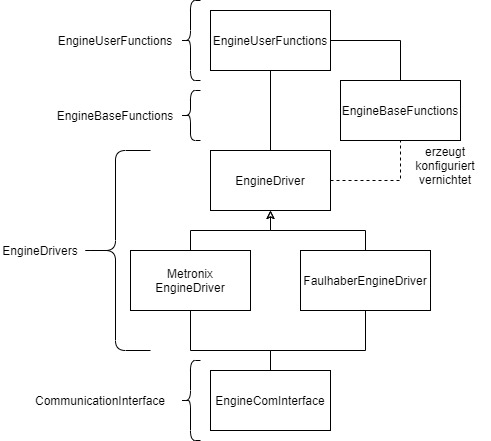
\includegraphics[width=1\textwidth]{img/ArchitekturFactory.jpg} 
   \caption{Architektur durch Factory Entwurfsmuster}
  \label{fig:ArchitekturFactory.jpg}
\end{figure}

 
\onehalfspacing
\section{Evaluation}
In diesem Kapitel wird die Evaluation des Projekts beschrieben. Die Evaluation gliedert sich in zwei Bestandteile. Zuerst wird eine Nutzenanalyse durchgeführt. Mit dieser soll geprüft werden, welchen realen Nutzen das Projekt im späteren Einsatz liefert. Im zweiten Schritt wird das Ergebnis der Arbeit mit den erstellten Anforderungen aus Kapitel \dq \nameref{sec:Anforderungsdefinition}\dq~abgeglichen. 
	\subsection{Nutzen Analyse}
	Um zu bestimmen, welchen Nutzen die Einführung der Suite auf die Entwicklung eines Tests hat, werden zwei Kriterien verwendet. Als Erstes wird verglichen wie viele Zeilen Code durch die Verwendung der Testsuite im eigentlichen Testfile eingespart werden können. 
	Um zu bestimmen wie viele \ac{LOC} durch den Einsatz der Suite eingespart werden können, werden verschiedene bisherige Testfälle betrachtet. Hierbei handelt es sich um die Testfälle, welche in Tabelle \dq \nameref{tab:LOCTestfall}\dq~aufgeführt sind. 
	
\begin{table}[h]
\begin{center}
\begin{tabularx}{\textwidth}{|X|X|c|}
\hline
Name & Geräte & \ac{LOC} \\
\hline
CriticalSpeed & Faulhaber Motor & 659 \\
\hline
ExtendedFuncHFSinCos & Faulhaber Motor, Hiperface & 865 \\
\hline
MultiturnAngleVerification & Faulhaber Motor & 749 \\
\hline
\end{tabularx}
\end{center}
\caption{Auswertung \ac{LOC} pro Testfall \label{tab:LOCTestfall}}
\end{table}
In Tabelle \dq \nameref{tab:einsparung}\dq~sind die Testfälle, sowie deren \ac{LOC} bei Verwendung der Testsuite dargestellt:\newline
\begin{table}[h]
\begin{center}
\begin{tabularx}{\textwidth}{|X|c|c|c|}
\hline
Name & \ac{LOC} & Einsparung & Einsparung \% \\
\hline
CriticalSpeed & 659 & ca. 50 & 7,59 \\
\hline
ExtendedFuncHFSinCos & 865 & ca. 80 & 9,24 \\
\hline
MultiturnAngleVerification & 749 & ca. 35 & 4,67 \\
\hline
\end{tabularx}
\end{center}
\caption{Auswertung Einsparung \label{tab:einsparung}}
\end{table}

Zu erkennen ist hierbei, dass es in allen betrachteten Testfällen zu einer Reduzierung der \ac{LOC} kommt. Hierbei ist jedoch anzumerken, dass es sich bei den drei Testfällen nicht um Testfälle für den SKx handelt. Bei Testfällen für den SKx ist mit einer deutlich höheren Einsparung zu rechnen.
Der Hauptvorteil welcher sich durch die Anwendung der Suite ergibt ist jedoch eher im Bereich des Clean Code zu sehen. Durch die Suite wird die Verwendung der verschiedenen Hardwarekomponenten standardisiert und ausgelagert, was zu einem übersichtlicheren Testfile führt. Auch ist die Komplexität für den Entwickler selbst deutlich geringer, da dieser sich nicht mit der expliziten Implementierung zum Beispiel des Motortreibers auseinandersetzen muss.
	\subsection{Abgleich der Anforderungen}
	Die Anforderungen welche in \dq \nameref{sec:Anforderungsdefinition}\dq~definiert sind, werden hier mit der realen Implementierung abgeglichen. In den Tabellen \dq \nameref{tab:AbgleichF}\dq~und \dq  \nameref{tab:AbgleichNF}\dq~sind die Ergebnisse aufgeführt. Hierbei wird jeweils zwischen Kriterien \dq erfüllt\dq, \dq teilweise erfüllt\dq~und \dq nicht erfüllt\dq~unterschieden. Alle Anforderungen werden grundlegend erfüllt. Ausnahme hierbei sind die Anforderungen \dq F07\dq~und \dq NF03 \dq. Anforderung F07 ist nur teilweise erfüllt, da im Rahmen des Proof of Concept der Bereich der Spannungsversorgung zwar geplant, jedoch nicht implementiert wird. Weiterhin ist im Rahmen des Proof of Concept kein ausführliches Code Review vorgesehen, sodass Anforderung NF03 zwar umgesetzt, die Umsetzung jedoch noch nicht verifiziert ist.
	
\begin{table}[h]
\begin{center}
\begin{tabularx}{\textwidth}{|c|X|c|X|}
\hline
Nr. & Bezeichnung & Status & Bemerkung \\
\hline
F01 &Integration in Automated Testing @ GBC07 & erfüllt &  durch Verwendung von ITE als Sprache sowie entsprechende Architektur \\
\hline
F02 & Schnittstellen Config & erfüllt & Hiperface Funktionalität vollständig implementiert \\
\hline
F03 & Diagnose Funktionalität & erfüllt & Hiperface Funktionalität vollständig implementiert \\
\hline
F04 & Core Funktionalität & erfüllt & Hiperface Funktionalität vollständig implementiert \\
\hline
F05 & Identifikation des DUT & erfüllt & Hiperface Funktionalität vollständig implementiert  \\
\hline
F06 & Hiperface Befehle & erfüllt & Hiperface Funktionalität vollständig implementiert \\
\hline
F07 & Error Codes & teilweise erfüllt & Hiperface Funktionalität vollständig implementiert, Motorfunktionalität vollständig implementiert, Spannungsversorgung geplant \\
\hline


\end{tabularx}
\end{center}
\caption{Abgleich Anforderungen funktional \label{tab:AbgleichF}}
\end{table}



\begin{table}[h]

\begin{center}

\begin{tabularx}{\textwidth}{|c|X|c|X|}

\hline
Nr. & Bezeichnung & Status & Bemerkung \\
\hline
NF01 & Externes Equipment & erfüllt & Einbinden von bisher vorhandenem Equipment geplant und teilweise implementiert, durch geplante Architektur ist das Einbinden weiterer HW möglich \\
\hline
NF02 & Universell einsetzbar & erfüllt & Durch geplante Architektur ist ein Einsatz auch in andern Projekten möglich, die einzelnen Module sind so gekapselt das sie wiederverwendet werden können. \\
\hline
NF03 & Coding Guidelines & teilweise erfüllt & Die Coding Guidelines werden beachtet. Jedoch fand bis jetzt kein entsprechendes Refactoring des Codes statt, um dies zu verifizieren. \\
\hline


\end{tabularx}
\caption{Anforderungen nicht-funktional \label{tab:AbgleichNF}}
\end{center}
\end{table}

	

\onehalfspacing
\section{Fazit / Ausblick}
In diesem Kapitel wird rückwirkend auf das Projekt eingegangen. Der Ablauf des Projekts wird kritisch reflektiert. Im weiteren Verlauf des Kapitels wird auf den zukünftigen Verlauf des Projekts eingegangen.
\subsection{Fazit}
Ziel dieser Arbeit war es eine Testsuite für die anstehende Portierung des SKx zu erstellen. Die Testsuite soll den Entwickler von Softwaretests bei seiner Aufgabe unterstützen und somit den Prozess beschleunigen. Die Testsuite sollte in das Projekt Automated Testing @ GBC07 integriert werden.
Zu Beginn des Projektes wurde ein Überblick über die verschiedenen Softwaretests geschaffen. Als Herausforderung hierbei stellte sich heraus, dass es noch keine Dokumentation der SKx Softwaretests gibt. Aus diesem Grund wurde auf die Dokumentation der Softwaretests am SEY zurückgegriffen. Die verschiedenen Softwaretests wurden nach definierten Kriterien analysiert und geprüft welche von ihnen sich mit der Suite abdecken lassen. Hierbei lag das Augenmerk auf der Automatisierbarkeit der Tests. Die in diesem Arbeitsschritt identifizierten Tests wurden im Anschluss geclustert und herausgearbeitet welche Hardware Komponenten verwendet werden. Aus den erarbeiteten Informationen wurde Anforderungen an das Projekt definiert und diese im Anschluss mit den Kunden abgestimmt. Die Requirements wurden hierbei in funktional und nicht-funktionale unterteilt. Die Analyse- und Konzeptionsphase zog sich real deutlich länger, als ursprünglich geplant. Grund hierfür war die aufwendige Analyse der Testfälle. In der folgenden Konzeptionsphase wurden zuerst die bisher vorhandenen Softwarekomponenten (Motor-, Hiperfacetreiber etc.) analysiert. Hier lag das Augenmerk darauf, zu identifizieren welche Teile der bisherigen Software eventuell wiederverwendet werden können und welche Architektur bisher verwendet wurde. Im zweiten Teil der Kozeptionierung erfolgte die Erstellung einer entsprechenden neuen. Hierfür wurden verschiedene Architekturmodelle (MVC, Pipe-Filter, Schichtenarchitektur) verglichen und das am Besten geeignete Modell ausgewählt. Das Ergebnis der Konzeption ist eine vier-Schichtarchitektur. Im Zuge der Konzeptionsphase wurde darüber hinaus eine wirtschaftliche Betrachtung des Projekts durchgeführt. Diese gestaltet sich jedoch schwierig, da sich nur schwer abschätzen lässt, welchen realen finanziellen Vorteil das Projekt in Zukunft bringen wird.
In der folgenden Implementierungsphase wurde ein Teil des Konzepts im Rahmen eines Proof of Concept umgesetzt. Die Programmierung erfolgte hierbei in der durch SICK entwickelten Programmiersprache ITE. Durch die Verwendung von ITE kam es bereits während der Konzeption zu verschiedenen Herausforderungen, da sich mit ihr gewisse Konstrukte wie zum Beispiel Interfaces nicht wie in andern objektorientierten Sprachen abbilden lassen. Durch diese Herausforderung konnten nicht alle architektonischen Probleme mit bekannten Entwurfsmustern gelöst werden.
Nach der prototypischen Implementierung wurden im Rahmen der Validierung drei verschiedene Testfiles  und die Auswirkung der Testsuite auf die Anzahl der benötigten Codezeilen untersucht. Trotz des Umstandes, dass es sich beim Proof of Concept lediglich um eine Teilimplementierung handelt, konnten hier bereits passable Ergebnisse erzielt werden. Weiterhin wurde das Ergebnis des Projekts mit den definierten Anforderungen abgeglichen, wobei diese weitestgehend erfüllt wurden.
\subsection{Ausblick}
Nachdem es sich im Rahmen dieser Arbeit nur um eine Proof of Concept Implementierung handelt, wird die tatsächliche Implementierung im Rahmen des Portierungsprojekt voraussichtlich fortgeführt werden. Hierbei kann davon ausgegangen werden, dass die in der Arbeit erstellten Konzepte und die darin enthaltene Architektur umgesetzt wird. Die bisher entwickelten Softwarekomponenten können hierfür weiterverwendet werden. Ein Refactoring, sowie ausführliche Tests sollten jedoch noch durchgeführt werden, um den Code zu verifizieren. Von Vorteil wäre eine enge Zusammenarbeit mit dem für die Portierung zuständigen Softwareentwickler. Nach Erstellung des konkreten Testplans durch den Entwickler müssen eventuell noch kleinere Änderungen an den \dq UserFunctions\dq~vorgenommen werden. Jedoch ist dies aufgrund der gewählten Architektur einfach möglich. Weiterhin muss die Logging Funktion, sowie die Ansteuerung der verschiedenen Netzteile implementiert werden. Durch die gewählte Architektur ist das Projekt auch für weitere Hardware, oder Softwareschnittstellen erweiterbar. So können zum Beispiel sehr schnell und komfortabel weitere Motoren eingebunden werden.  

\pagenumbering{Roman}
\onehalfspacing
\section{Literatur}
	\bibliography{Literatur}
\onehalfspacing
\section{Anhang}







%=====Anhang====



\end{document}
